%==================== main.tex (LuaLaTeX / IEEEtran, conference) ====================
\documentclass[conference]{IEEEtran}

% ---- Fonts (LuaLaTeX-friendly; neat Times-like look) ----
\usepackage{fontspec}
\usepackage{newtxtext,newtxmath}

% ---- Figures / tables / subfig ----
\usepackage{graphicx}
\graphicspath{{figures/}}
\usepackage[font=footnotesize]{subfig}
\usepackage{booktabs}
\usepackage{siunitx}
\sisetup{detect-all=true,detect-weight=true}

% ---- Colors & TikZ (for simple process/cross-section diagrams) ----
\usepackage{xcolor}
\usepackage{tikz}
\usetikzlibrary{positioning,arrows.meta}

% ---- Hyperref (after most packages) ----
\usepackage[hidelinks]{hyperref}
\usepackage{cite}

% ---- Convenience macros ----
\newcommand{\TZDBFig}{fig3_tzdb.png}
\newcommand{\TDDBCdfFig}{fig4_tddb_cdf.png}
\newcommand{\TDDBWeibullFig}{fig4_tddb_weibull.png}
\newcommand{\ENDURANCEFig}{fig5_endurance.png}
\newcommand{\RETENTIONFig}{fig6_retention.png}

\newcommand{\um}{\ensuremath{\mu\mathrm{m}}}
\newcommand{\degreeC}{\ensuremath{^\circ\! \mathrm{C}}}

\begin{document}

\title{Low-Cost Integration of 1.8-V FeFET on 0.18-\um{} CMOS:\\
\Large +1 Mask and a Single ALD Tool, with Reliability Assessment}

\author{
\IEEEauthorblockN{Shinichi Samizo}
\IEEEauthorblockA{Independent Semiconductor Researcher\\
Former Engineer at Seiko Epson Corporation\\
Email: shin3t72@gmail.com \quad GitHub: \url{https://github.com/Samizo-AITL}}
}

\maketitle

\begin{abstract}
Ferroelectric FETs (FeFETs) are promising CMOS-compatible nonvolatile memories. This paper demonstrates a \SI{1.8}{V} FeFET module integrated on a legacy \SI{0.18}{\micro\meter} CMOS process with only one additional mask and a single ALD tool. Fabricated devices show endurance exceeding $10^{5}$ program/erase cycles and retention longer than 10~years at \SI{85}{\celsius}. Reliability was characterized on FeCAP/FeFET structures: time-zero dielectric breakdown (TZDB), time-dependent dielectric breakdown (TDDB), endurance, and retention. The approach provides a cost-effective path to extend mature-node lifetimes and to enable embedded NVM for automotive/industrial/IoT, where high-temperature retention remains the key limiter.
\end{abstract}

\section{Introduction}
Ferroelectric HfO\textsubscript{2}-based memories attract attention as CMOS-compatible NVMs~\cite{boscke2011,mueller2012,mikolajick2019,mueller2015}. While many works target advanced nodes, mature nodes (e.g., \SI{0.18}{\micro\meter}) remain workhorses in automotive/industrial sectors for cost and longevity. \emph{This work contributes:} (i) a +1 mask low-cost module, (ii) only one ALD tool added to the line, (iii) a yield-friendly SRAM+FeFET system usage model, and (iv) comprehensive reliability evidence (TZDB, TDDB, endurance, retention) on FeCAP/FeFET.

\section{Process Integration}
Baseline is a \SI{0.18}{\micro\meter} CMOS platform (1.8~V core, optional 3.3~V I/O). The FeFET module is inserted after poly definition and salicide/RTA, requiring minimal line modification.

\subsection{Process Flow}
Fig.~\ref{fig:flow} sketches the insertion flow. Only one extra mask step (ferroelectric gate) and one ALD tool are introduced; all other steps reuse existing modules (TiN, RTA, BEOL).

\begin{figure}[t]
  \centering
  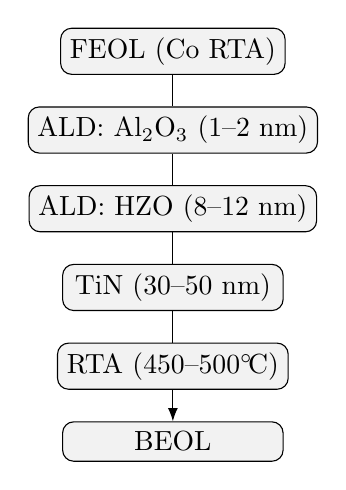
\begin{tikzpicture}[
    box/.style={draw,rounded corners,align=center,minimum width=28mm,minimum height=5mm},
    node distance=4mm
  ]
    \node[box,fill=gray!10] (feol) {FEOL (Co RTA)};
    \node[box,below=of feol,fill=gray!10] (ald1) {ALD: Al$_2$O$_3$ (1--2 nm)};
    \node[box,below=of ald1,fill=gray!10] (ald2) {ALD: HZO (8--12 nm)};
    \node[box,below=of ald2,fill=gray!10] (tin)  {TiN (30--50 nm)};
    \node[box,below=of tin,fill=gray!10] (rta)  {RTA (450--500\degreeC)};
    \node[box,below=of rta,fill=gray!10] (beol) {BEOL};
    \draw[-{Latex}] (feol) -- (ald1) -- (ald2) -- (tin) -- (rta) -- (beol);
  \end{tikzpicture}
  \caption{Process flow for FeFET integration (single ALD tool).}
  \label{fig:flow}
\end{figure}

\subsection{Cross Section}
The FeFET stack uses HZO/Al\textsubscript{2}O\textsubscript{3}/TiN. A thin Al\textsubscript{2}O\textsubscript{3} interlayer suppresses wake-up/fatigue while stabilizing the ferroelectric phase window.

\begin{figure}[t]
  \centering
  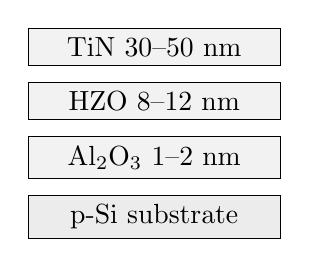
\begin{tikzpicture}[
    box/.style={draw,align=center,minimum width=32mm},
    node distance=2mm
  ]
    \node[box,fill=gray!15] (psub) {p-Si substrate};
    \node[box,fill=gray!10,above=of psub] (al2o3) {Al$_2$O$_3$ 1--2 nm};
    \node[box,fill=gray!10,above=of al2o3] (hzo) {HZO 8--12 nm};
    \node[box,fill=gray!10,above=of hzo] (tin) {TiN 30--50 nm};
  \end{tikzpicture}
  \caption{Schematic cross section of HZO/Al$_2$O$_3$/TiN FeFET stack.}
  \label{fig:xsec}
\end{figure}

\section{Devices and Methods}
Test structures include FeCAPs (flat/comb) and \SI{100}{\micro\meter} FeFET cells. Programming used $\pm$2.3--2.7~V, 1--50~\si{\micro\second} pulses. A Keysight B1500A with a manual probe station was used.

\textbf{Protocols:}
TZDB: DC ramp $\approx$~\SI{0.1}{V/s} at RT--\SI{125}{\celsius}. \\
TDDB: constant-voltage stress at $\pm$2.3/2.5/2.7~V, \SI{85}{\celsius} and \SI{125}{\celsius}. \\
Weibull fitting. \\
Endurance: $\pm$2.5~V, \SI{10}{\micro\second}, 10~kHz up to $10^{5}$ cycles. \\
Retention: \SI{25}{\celsius}, \SI{85}{\celsius}, \SI{125}{\celsius} with Arrhenius extrapolation.

\section{Results: Reliability}
For readability, results are split across multiple figures of identical width.

\subsection{Time-Zero Dielectric Breakdown (TZDB)}
\begin{figure}[t]
  \centering
  \includegraphics[width=0.95\linewidth]{\TZDBFig}
  \caption{TZDB distributions of FeCAPs. Early-failure tails imply defect-driven paths.}
  \label{fig:tzdb}
\end{figure}

\subsection{TDDB under Constant-Voltage Stress}
\begin{figure}[t]
  \centering
  \includegraphics[width=0.95\linewidth]{\TDDBCdfFig}
  \caption{TDDB cumulative failure probability (CDF) under multiple stresses (\SI{85}{\celsius}/\SI{125}{\celsius}, $\pm$2.3/2.5/2.7~V).}
  \label{fig:tddb_cdf}
\end{figure}

\begin{figure}[t]
  \centering
  \includegraphics[width=0.95\linewidth]{\TDDBWeibullFig}
  \caption{TDDB Weibull plots with slope $\beta \approx 1.3$ and scale $\eta$.}
  \label{fig:tddb_weibull}
\end{figure}

\subsection{Endurance}
\begin{figure}[t]
  \centering
  \includegraphics[width=0.95\linewidth]{\ENDURANCEFig}
  \caption{Endurance characteristics ($\Delta V_\mathrm{th}$ vs.\ cycles). Up to $10^{5}$ cycles; memory window shrinks 20--30\%.}
  \label{fig:endurance}
\end{figure}

\subsection{Retention}
\begin{figure}[t]
  \centering
  \includegraphics[width=0.95\linewidth]{\RETENTIONFig}
  \caption{Retention summary (CDF and/or Arrhenius extrapolation). Prediction: $>$10~y @ \SI{85}{\celsius}, months @ \SI{150}{\celsius}.}
  \label{fig:retention}
\end{figure}

\subsection{Model Fits}
Weibull slope $\beta \approx 1.3$; Arrhenius activation $E_a \approx 0.78$~eV (2.3~V), 0.84~eV (2.5~V), 0.88~eV (2.7~V). A compact endurance fit is
\[
\Delta V_\mathrm{th}(N)=1.12 - 0.05\log_{10}N.
\]
Retention extrapolation with $E_a \approx 1.1$~eV supports long retention at $\le \SI{85}{\celsius}$.

\section{System Architecture (SRAM + FeFET)}
\begin{figure}[t]
  \centering
  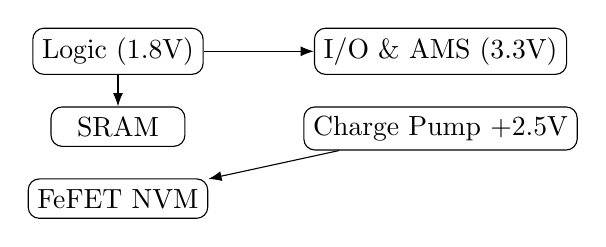
\begin{tikzpicture}[
    box/.style={draw,rounded corners,align=center,minimum width=17mm,minimum height=5mm},
    node distance=4mm
  ]
    \node[box] (logic) {Logic (1.8V)};
    \node[box,below=of logic] (sram) {SRAM};
    \node[box,right=14mm of logic] (io) {I/O \& AMS (3.3V)};
    \node[box,below=of sram] (nvm) {FeFET NVM};
    \node[box,below=of io] (pump) {Charge Pump +2.5V};
    \draw[-{Latex}] (pump) -- (nvm);
    \draw[-{Latex}] (logic) -- (io);
    \draw[-{Latex}] (logic) -- (sram);
  \end{tikzpicture}
  \caption{System architecture with SRAM backup to FeFET.}
  \label{fig:arch}
\end{figure}

\begin{figure}[t]
  \centering
  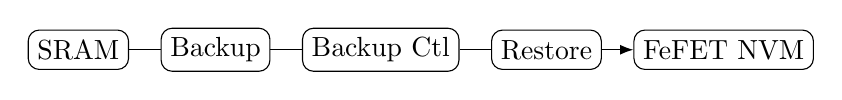
\begin{tikzpicture}[
    box/.style={draw,rounded corners,align=center,minimum width=12mm,minimum height=5mm},
    node distance=4mm
  ]
    \node[box] (sram) {SRAM};
    \node[box,right=of sram] (bkp) {Backup};
    \node[box,right=of bkp] (ctrl) {Backup Ctl};
    \node[box,right=of ctrl] (rst) {Restore};
    \node[box,right=of rst] (nvm) {FeFET NVM};
    \draw[-{Latex}] (sram) -- (bkp) -- (ctrl) -- (rst) -- (nvm);
  \end{tikzpicture}
  \caption{Backup/restore flow between SRAM and FeFET.}
  \label{fig:flow_sram}
\end{figure}

\section{Discussion}
For industrial/consumer embedded NVM, the HZO/Al$_2$O$_3$/TiN stack is sufficient. For high-temperature automotive, improvements are recommended:

\textbf{Interlayer (IL) optimization:} Al$_2$O$_3$ thickness/composition tuning to mitigate wake-up/fatigue and reduce leakage.\\
\textbf{Crystallinity control:} RTA window and TiN work-function engineering to stabilize ferroelectric phase and reduce variation.\\
\textbf{Defect mitigation:} Precursor purity, ALD purge optimization, and post-deposition anneal to suppress oxygen-vacancy paths (helps TDDB/retention).\\
\textbf{Circuit assists:} Verify-and-rewrite (background refresh at high-$T$), ECC, and adaptive write pulse shaping to slow window loss.\\
\textbf{Array architecture:} Redundancy/repair and SRAM+FeFET hybrid usage to keep frequent writes on SRAM, reducing FeFET stress.

\section{Conclusion}
We realized a +1 mask FeFET module on \SI{0.18}{\micro\meter} CMOS with only one additional ALD tool. Devices exhibit $>10^{5}$ cycles and $>10$~year retention at \SI{85}{\celsius}, verified by TZDB/TDDB/endurance/retention analyses. The method extends mature-node lifetime and enables cost-effective embedded NVM for automotive/industrial/IoT.

\section*{Acknowledgment}
The author thanks collaborators for helpful discussions.

\begin{thebibliography}{00}
\bibitem{boscke2011}
T. Böscke \textit{et al.}, “Ferroelectricity in hafnium oxide thin films,” \textit{Appl. Phys. Lett.}, vol.~99, p.~102903, 2011.
\bibitem{mueller2012}
J. Müller \textit{et al.}, “Ferroelectricity in simple binary ZrO$_2$ and HfO$_2$,” \textit{Appl. Phys. Lett.}, vol.~99, p.~112901, 2012.
\bibitem{mikolajick2019}
T. Mikolajick \textit{et al.}, “Ferroelectric hafnium oxide for memory applications,” \textit{J. Appl. Phys.}, vol.~125, p.~204103, 2019.
\bibitem{mueller2015}
J. Müller \textit{et al.}, “Ferroelectricity in HfO$_2$-based thin films: devices and applications,” \textit{IEEE Trans. Electron Devices}, vol.~62, no.~12, pp.~4158--4166, 2015.
\bibitem{park2014}
J. Park \textit{et al.}, “Endurance of FeFETs,” \textit{IEEE Electron Device Lett.}, vol.~41, no.~5, pp.~711--714, 2014.
\bibitem{nam2003}
H. Nam \textit{et al.}, “Time-dependent dielectric breakdown in HfO$_2$,” \textit{IEEE Trans. Device Mater. Rel.}, vol.~3, no.~4, pp.~132--136, 2003.
\bibitem{yamazaki2018}
Y. Yamazaki \textit{et al.}, “Retention of HZO-based FeCAP/FeFET,” \textit{Jpn. J. Appl. Phys.}, vol.~57, 04BF07, 2018.
\end{thebibliography}

\section*{Biography}
Shinichi Samizo has over 25 years of experience in semiconductor process integration and actuator development. After studying control theory and EM modeling in academia, he joined Seiko Epson in 1997 and worked on 0.35--0.18~\um{} CMOS logic/memory/HV integration, DRAM, and LCD drivers. Later he contributed to PZT actuator development and the PrecisionCore inkjet head. He is currently an independent researcher, publishing educational materials via the “Project Design Hub”.

\end{document}
